%------------------------------------------------------------------------------
% Introduction
%------------------------------------------------------------------------------

\section{Introduction}
\label{sec:intro}

Video diffusion models (VDMs) have become a powerful tool for animating a
static image into a short flythrough~\cite{wan2025,viewcrafter,gen3c,seva}.
When the goal is not just a video but an \emph{explorable 3D scene}, however,
a fundamental problem emerges: the generated frames are not 3D-consistent.
Geometric foundation models (GFMs) such as DepthAnything-3~\cite{da3} lift
each frame into a per-pixel point cloud, but because the VDM hallucinates
content independently per frame, the resulting point clouds do not overlap
into a single surface --- a phenomenon called \emph{generative
drift}~\cite{hoellein2026worldreconstruction}. Recent work reconstructs a
consistent 3D world from these inconsistent views by non-rigidly aligning the
per-frame point clouds into a canonical frame~\cite{hoellein2026worldreconstruction}.

In this paper we ask a complementary question: \emph{can the input image
itself serve as a 3D-stability prior?} We focus on the case where the input is
a \textbf{human oil painting}. Oil paintings are an attractive input modality
for 3D world generation: they are user-authored, stylistically rich, and ---
crucially --- encode a deliberate compositional structure. The artist has
already chosen the depth layout, the brush-stroke arrangement, and the
focal-accent placement. We show that this structure can be lifted into a
canonical-frame prior that constrains both the video generation and the 3D
reconstruction, dramatically reducing generative drift.

\textbf{Contributions.} We propose Paint2World, a pipeline that turns a single
oil painting into a 3D-consistent flythrough video and a 3D Gaussian Splatting
scene (Fig.~\ref{fig:teaser}). Our contributions are:
\begin{itemize}
\item An \textbf{object-level scene canvas} built directly from the painting:
a depth-aware image-segmentation front-end decomposes the artwork into
objects, a TripoSplat-style triplane-to-Gaussian decoder generates each
object in 3D from its painting view and depth-warped side views, and the
objects are wired into a 3D \emph{spatial-dependency graph} (supports /
occludes / adjacent / rests-on-ground) whose contacts are physically
resolved on a fitted ground plane (\S\ref{sec:stage-object}).
\item A \textbf{painting-conditioned video generation stage} with three
3D-stability controls: a depth-warp geometry ControlNet signal composited
from the scene canvas, a stroke-consistency temporal-attention bias, and a
temporal-consistency guidance term (\S\ref{sec:stage0}).
\item A \textbf{painting-anchored non-rigid alignment} that initialises the
canonical frame from the painting's estimated geometry and weights each
generated point by a depth-warp consistency score, allowing the scene to
plausibly extend beyond the painting's frustum while suppressing drift within
it (\S\ref{sec:stage1}).
\item A \textbf{stroke-coherent, object-rigid 3D Gaussian Splatting
objective}: the painting's brush-stroke segmentation is transferred onto the
3D Gaussians so each stroke remains a coherent 3D patch, while per-object
SE(3) anchors move objects as wholes and a relation-preservation loss keeps
the canvas's spatial dependencies intact during optimisation, together with a
painting-view reconstruction loss that ties the scene back to the input
artwork (\S\ref{sec:stage3}).
\end{itemize}
We demonstrate that Paint2World produces 3D-consistent, explorable scenes from
oil paintings and that the object-level canvas and each stability mechanism
measurably improve 3D consistency, painting fidelity, and scene-structure
preservation (\S\ref{sec:experiments}).

\begin{figure*}[t]
\centering
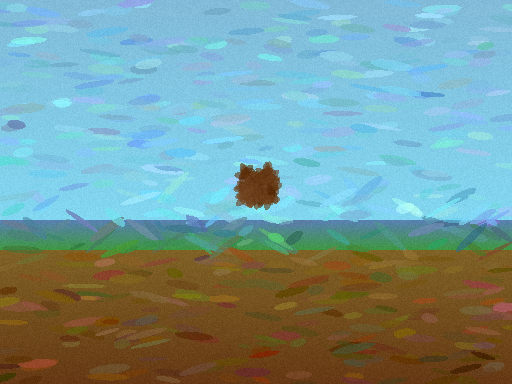
\includegraphics[width=0.48\linewidth]{figures/teaser_painting.png}\hfill
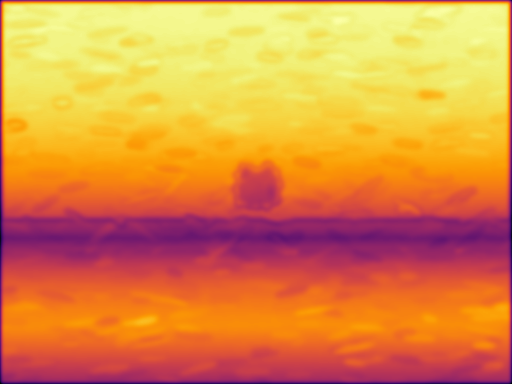
\includegraphics[width=0.48\linewidth]{figures/teaser_depth.png}
\caption{\textbf{Paint2World.} Given a single human oil painting (left), we
estimate its depth, normals, brush-stroke segmentation, and object
segmentation (Stage -1); construct an explicit 3D scene canvas by generating
each segmented object with a TripoSplat-style triplane-to-Gaussian decoder
and wiring the objects into a spatial-dependency graph (Stage -0.5); generate
a 3D-stable flythrough video whose geometry is anchored to the canvas
(Stage 0); non-rigidly align the generated frames into a painting-initialised
canonical point cloud (Stage 1); and train a stroke-coherent, object-rigid 3D
Gaussian Splatting scene that reproduces the painting from its viewpoint
(Stage 3.2).}
\label{fig:teaser}
\end{figure*}
